We benchmark MARL algorithms in four customized \textit{ComplexOvercooked} layouts with increased difficulty (Figure \ref{fig:exp_layouts}): \textit{Supereasy}, \textit{2playerhard}, \textit{4playereasy}, \textit{4playersplit} (Figure\ref{fig:exp_layouts}). \textit{supereasy} is a layout with static objective (i.e.,  \textit{AClemoncookedfish}) that supports two players playing. \textit{2playerhard}, \textit{4playereasy} and \textit{4playersplit} support four types of orders (i.e., \textit{Cookedfish}, \textit{AClemoncookedfish}, \textit{Cookedbeefhamburger} and \textit{ACtomatocookedbeefhamburger}) among which two random orders will be generated simultaneously in the task menu every 200 timesteps. \\
\begin{figure}[H]
    \centering
    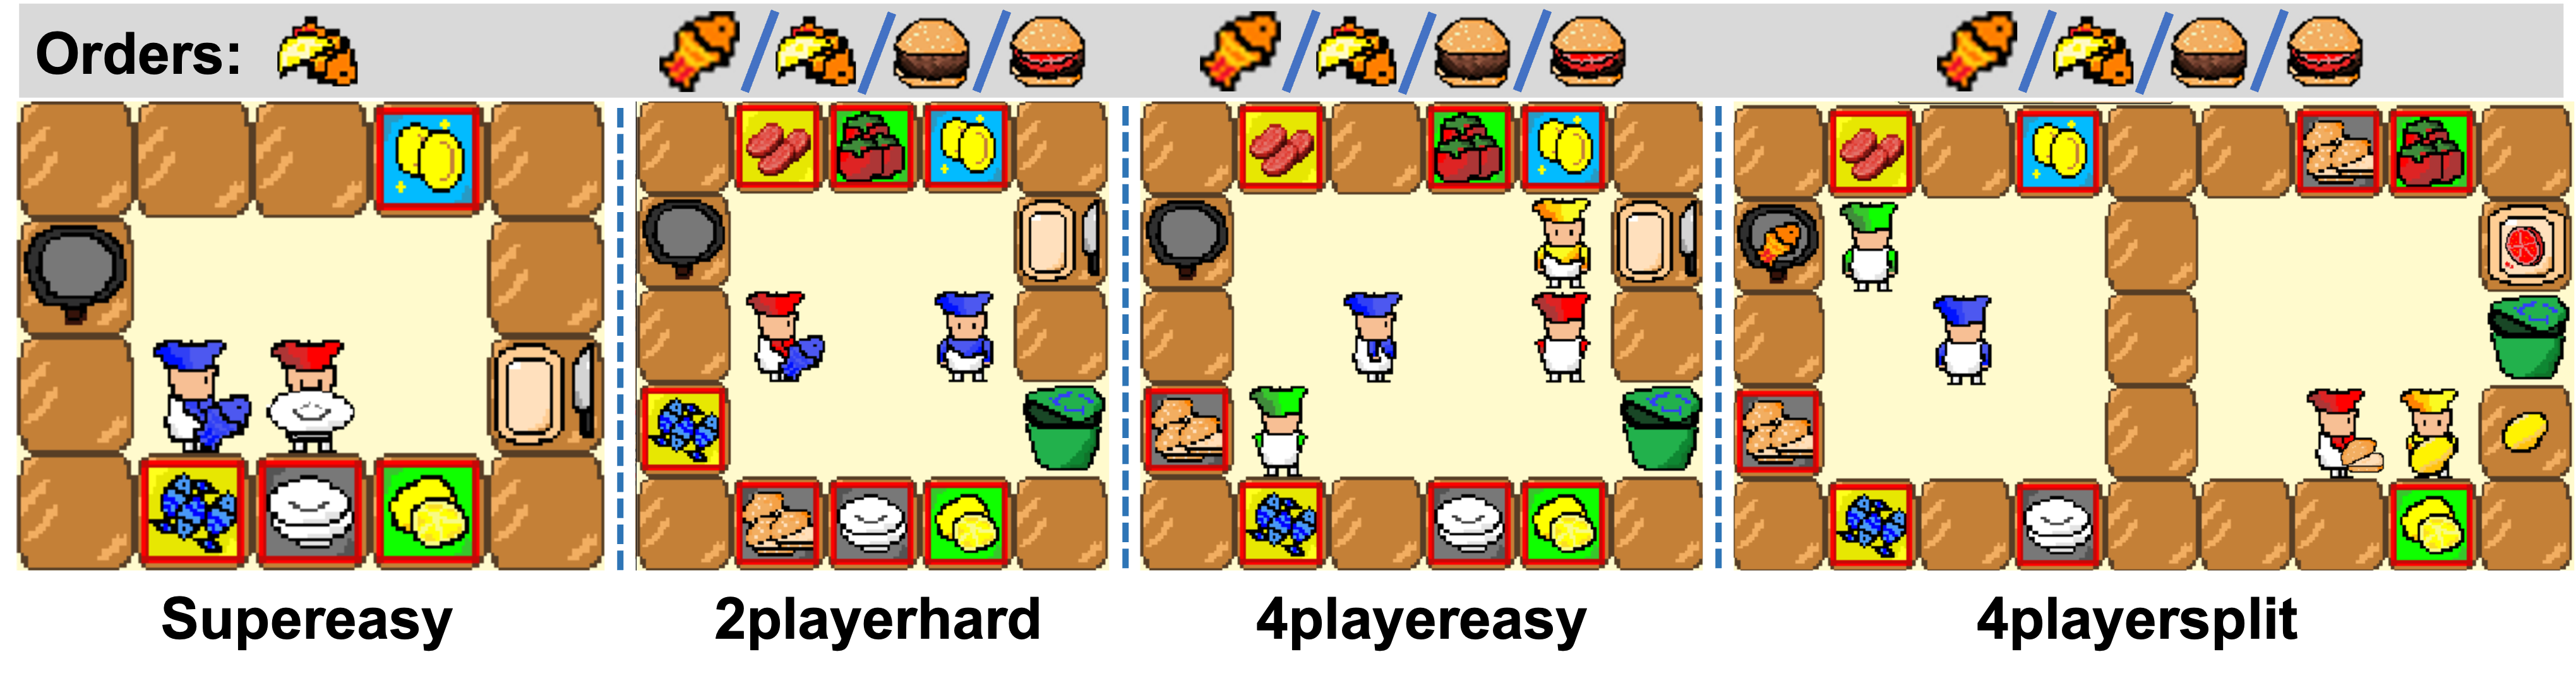
\includegraphics[width=\linewidth]{Figures/4layouts.png}
  \caption{Layouts used in our experiments. From left to right, the difficulty gradually increases. The layout \textit{4playereasy} and \textit{4playersplit} supports four agents playing, and it offers a greater variety of tasks and supports four player interface.}
\label{fig:exp_layouts} 
\end{figure} 
\noindent\textbf{MARL algorithms} \ We use IPPO (independent PPO), VDN and IQL (independent Q-Learning) algorithms. The implementation of these algorithms can be referenced in \cite{papoudakis2020benchmarking}. Hyperparameters can be found in Appendix \ref{appendix:hyper}. \\
\noindent\textbf{Training} \ In each layout, we train MARL agents for 2e7 steps and record average returns over 5 random seeds (Figure \ref{fig:training_curves}). From the training curves we can see that on-policy and off-policy algorithms can converge, but standard deviations seem to be large. In addition, when facing multiple objectives (i.e.,  Figure \ref{fig:training_curves}: b, c, d), the performance of the agents is suboptimal, and it is difficult for them to converge to an ideal reward.

\begin{figure}[H]
    \centering
        \subfloat[Supereasy]{
        \includegraphics[width=0.5\linewidth]{Figures/overcooked2_supereasy_return_mean_True.pdf}}
        \subfloat[2playerhard]{
        \includegraphics[width=0.5\linewidth]{Figures/overcooked2_2playerhard_return_mean_True.pdf}}
        \hfill
        \subfloat[4playereasy]{
        \includegraphics[width=0.5\linewidth]{Figures/overcooked2_4playereasy_return_mean_True.pdf}}
        \subfloat[4playersplit]{
        \includegraphics[width=0.5\linewidth]{Figures/overcooked2_4playersplit_return_mean_True.pdf}}  
    \caption{Training curves of MARL algorithms in four game layouts of \textit{ComplexOvercooked}. The shaded areas denote the standard deviation over five random seeds.}
    \label{fig:training_curves}
\end{figure}
